\chapter{Literature Review}

This chapter presents a comprehensive review of existing literature, encompassing both theoretical frameworks that explain technology adoption and empirical studies that provide quantitative context for the ``War on Plastic.''

\section{Theoretical Frameworks}

The rapid displacement of physical cards by digital interfaces is not merely a technological upgrade; it is a behavioral phenomenon deeply rooted in user psychology and social dynamics. To rigorously analyze this shift, this study employs two seminal theoretical frameworks.

\subsection{Technology Acceptance Model (TAM)}

Proposed by Fred Davis in 1989, the Technology Acceptance Model (TAM) is one of the most widely cited frameworks in information systems research. It posits that two primary factors influence an individual's behavioral intention to use a new technology: \textbf{Perceived Usefulness (PU)} and \textbf{Perceived Ease of Use (PEOU)}.

\subsubsection{Perceived Usefulness (PU) in Financial Technology}

PU is defined as ``the degree to which a person believes that using a particular system would enhance his or her job performance'' (Davis, 1989). In the context of consumer payments, ``job performance'' translates to ``transactional efficiency'' and ``financial utility.''

\begin{itemize}
    \item \textbf{Liquidity Management:} The primary utility of ``Credit on UPI'' is the access to liquidity at the bottom of the pyramid. Previously, a user could not use credit to buy vegetables or pay a neighborhood barber.
    \item \textbf{Rewards on Micro-Spend:} Indian consumers are highly value-conscious. Traditional credit cards offered rewards, but only at large merchants. Credit on UPI extends this reward mechanism to every scan.
\end{itemize}

\subsubsection{Perceived Ease of Use (PEOU) and the ``Scan'' Paradigm}

PEOU refers to ``the degree to which a person believes that using a particular system would be free of effort'' (Davis, 1989).

\begin{itemize}
    \item \textbf{Friction Reduction:} The physical act of using a credit card involves friction: locating the wallet, removing the card, inserting it into a machine, and entering a PIN. The ``Scan and Pay'' workflow is perceived as significantly faster.
    \item \textbf{The ``Wallet-less'' Experience:} The integration of credit into the UPI app allows for a truly wallet-less existence. The ``card'' is now software, always present on the device.
\end{itemize}

\subsection{Unified Theory of Acceptance and Use of Technology (UTAUT)}

Venkatesh et al. (2003) formulated the UTAUT model to unify eight existing theories of technology acceptance. It identifies four key determinants of usage intention: \textbf{Performance Expectancy}, \textbf{Effort Expectancy}, \textbf{Social Influence}, and \textbf{Facilitating Conditions}.

\subsubsection{Performance Expectancy (PE): Speed and Economic Utility}

PE is defined as the degree to which an individual believes that using the system will help them attain gains in job performance.

\begin{itemize}
    \item \textbf{Instant Settlement:} For the merchant, ``performance'' is measured in settlement speed. UPI transactions settle in real-time (IMPS), giving the merchant instant access to funds.
    \item \textbf{Success Rates:} The reliability of the UPI infrastructure contributes to high performance expectancy.
\end{itemize}

\subsubsection{Social Influence (SI): The Network Effect of QR Codes}

SI reflects the extent to which an individual perceives that important others believe they should use the new system.

\begin{itemize}
    \item \textbf{Vernacular Adoption:} In India, ``Google Pay'' or ``Paytm'' has become a verb. The visual dominance of QR codes creates a strong normative pressure.
    \item \textbf{Demographic Drivers:} Data reveals that \textbf{45\%} of UPI-enabled credit card users are under the age of 30. This demographic is highly sensitive to peer behavior.
\end{itemize}

\subsubsection{Facilitating Conditions (FC): Smartphone Penetration and DPI}

FC refers to the existence of technical and organizational infrastructure to support the use of the system.

\begin{itemize}
    \item \textbf{Digital Public Infrastructure (DPI):} The ``JAM Trinity'' (Jan Dhan-Aadhaar-Mobile) provided the foundational rails.
    \item \textbf{Regulatory Support:} The RBI's specific intervention to allow RuPay credit cards on UPI was the ultimate facilitating condition.
    \item \textbf{Device Availability:} With over 600 million smartphones in India, the hardware required to ``accept'' the technology is already in the user's hand.
\end{itemize}

\section{Empirical Studies}

\subsection{Global Parallels: The ``Pix'' Revolution in Brazil}

The most direct corollary to India's UPI phenomenon is Brazil's \textbf{Pix} system, launched by the Central Bank of Brazil in late 2020.

\subsubsection{Duarte et al. (2022): The Substitution Effect}

In a seminal working paper titled \textit{``Instant Payments and the Demise of Cash,''} Duarte analyzed transaction data from 2020 to 2022. The study found a strong substitution effect between Pix and cash, but more interestingly, it observed a ``soft substitution'' for debit cards.

\begin{itemize}
    \item \textbf{Key Finding:} For transactions under BRL 50 (approx. \rupee 800), Pix usage surged while debit card swipes stagnated.
    \item \textbf{Relevance to India:} This mirrors the Indian micro-transaction economy. However, the study noted that \textit{credit card} usage remained resilient for high-value installments (BNPL), suggesting that ``Pay Later'' (Credit) defends its territory better than ``Pay Now'' (Debit).
\end{itemize}

\subsection{The Chinese Paradigm: Alipay vs. UnionPay}

China represents a mature market where QR codes (Alipay and WeChat Pay) have achieved near-total saturation, challenging the state-backed card network, UnionPay.

\subsubsection{Chen \& Zhang (2021): Platform Ecosystems}

Their research highlighted that the success of QR payments was not just about the payment mechanism but the ``Super App'' ecosystem. Users didn't just pay; they chatted, booked cabs, and ordered food within the same app.

\begin{itemize}
    \item \textbf{Inference:} Physical cards are ``dumb'' instruments; they only transmit payment data. Apps are ``smart'' ecosystems. This puts plastic cards at a severe disadvantage in terms of user engagement.
\end{itemize}

\subsection{Domestic Literature: The Indian Context}

\subsubsection{NITI Aayog (2023): Digital Payments Report}

The NITI Aayog report highlighted a crucial metric: \textbf{Volume vs. Value Divergence}.

\begin{quote}
    \textit{``While UPI accounts for 75\% of retail digital transaction volumes, credit cards still command a disproportionate share of transaction value.''}
\end{quote}

This finding underpins the current study's hypothesis: UPI wins on \textit{frequency} (buying milk), while Cards win on \textit{value} (buying a fridge). The integration of RuPay Credit on UPI is the bridge attempting to capture both.

\subsubsection{RBI Bulletin (April 2024): ``The Merchant Perspective''}

An RBI survey of Tier-3 merchants revealed that \textbf{88\%} of small retailers cited ``No MDR'' as the primary reason for preferring UPI over Cards. The study concluded that the cost of acceptance (MDR) is the single biggest barrier to the survival of the plastic card in the MSME sector.

\subsubsection{Bhattacharya (2023): Credit on UPI and Financial Inclusion}

Writing in the \textit{Economic and Political Weekly}, Bhattacharya analyzed the potential of Credit on UPI to democratize access to credit for underbanked populations. The study found that virtual credit issuance through UPI apps could reduce customer acquisition costs by up to 70\% compared to traditional physical card issuance.

\subsubsection{PwC India (2024): The Indian Payments Handbook}

The PwC report projected that by 2029, ``Credit on UPI'' could capture 15--20\% of the total credit card transaction value, primarily cannibalizing the mid-ticket segment (\rupee 2,000--\rupee 10,000).

\begin{figure}[htbp]
    \centering
    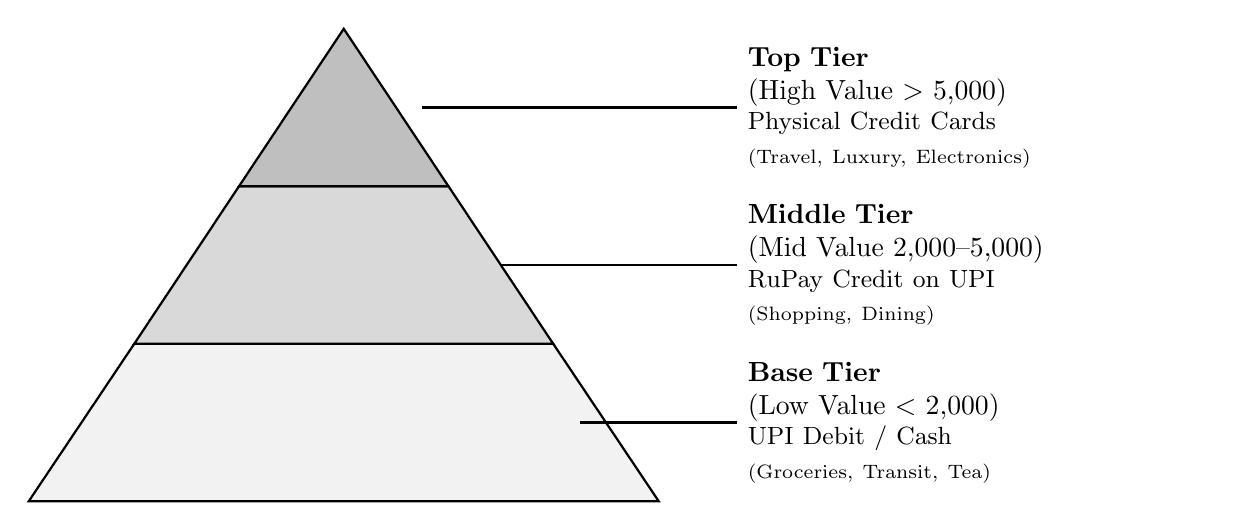
\begin{tikzpicture}
        % Define pyramid coordinates
        \coordinate (A) at (-4,0);
        \coordinate (B) at (4,0);
        \coordinate (C) at (0,6);

        % Define tier boundaries
        \coordinate (L1) at (-2.66, 2);
        \coordinate (R1) at (2.66, 2);
        \coordinate (L2) at (-1.33, 4);
        \coordinate (R2) at (1.33, 4);

        % Draw tiers with shading
        \filldraw[fill=gray!10, draw=black, thick] (A) -- (B) -- (R1) -- (L1) -- cycle;
        \filldraw[fill=gray!30, draw=black, thick] (L1) -- (R1) -- (R2) -- (L2) -- cycle;
        \filldraw[fill=gray!50, draw=black, thick] (L2) -- (R2) -- (C) -- cycle;

        % Labels on the right
        % Top Tier
        \draw[thick] (1, 5) -- (5, 5) node[right, align=left, text width=6cm] {
            \textbf{Top Tier} \\
            (High Value $>$ \rupee 5,000) \\
            \small Physical Credit Cards \\
            \scriptsize (Travel, Luxury, Electronics)
        };

        % Middle Tier
        \draw[thick] (2, 3) -- (5, 3) node[right, align=left, text width=6cm] {
            \textbf{Middle Tier} \\
            (Mid Value \rupee 2,000--\rupee 5,000) \\
            \small RuPay Credit on UPI \\
            \scriptsize (Shopping, Dining)
        };

        % Base Tier
        \draw[thick] (3, 1) -- (5, 1) node[right, align=left, text width=6cm] {
            \textbf{Base Tier} \\
            (Low Value $<$ \rupee 2,000) \\
            \small UPI Debit / Cash \\
            \scriptsize (Groceries, Transit, Tea)
        };

    \end{tikzpicture}
    \caption{Proposed Theoretical Segmentation of Payment Instruments}
    \label{fig:pyramid}
\end{figure}
